% +------------------------------------------------------------------------+
% | Reference manual page: APSS_implicit_function.tex
% +------------------------------------------------------------------------+
% | 02.06.2008   Pierre Alliez, Laurent Saboret, Gael Guennebaud
% | Package: Surface_reconstruction_3
% |
\RCSdef{\RCSAPSSimplicitfunctionRev}{$Id$}
\RCSdefDate{\RCSAPSSimplicitfunctionDate}{$Date$}
% |
\ccRefPageBegin
%%RefPage: end of header, begin of main body
% +------------------------------------------------------------------------+


\begin{ccRefClass}{APSS_implicit_function<GeomTraits, PointWithNormal_3>}

%% \ccHtmlCrossLink{}     %% add further rules for cross referencing links
%% \ccHtmlIndexC[class]{} %% add further index entries

\ccDefinition

% Insert image APSS.jpg/eps
\begin{center}
    \label{Surface_reconstruction_3-fig-APSS}
    % Image
    \begin{ccTexOnly}
        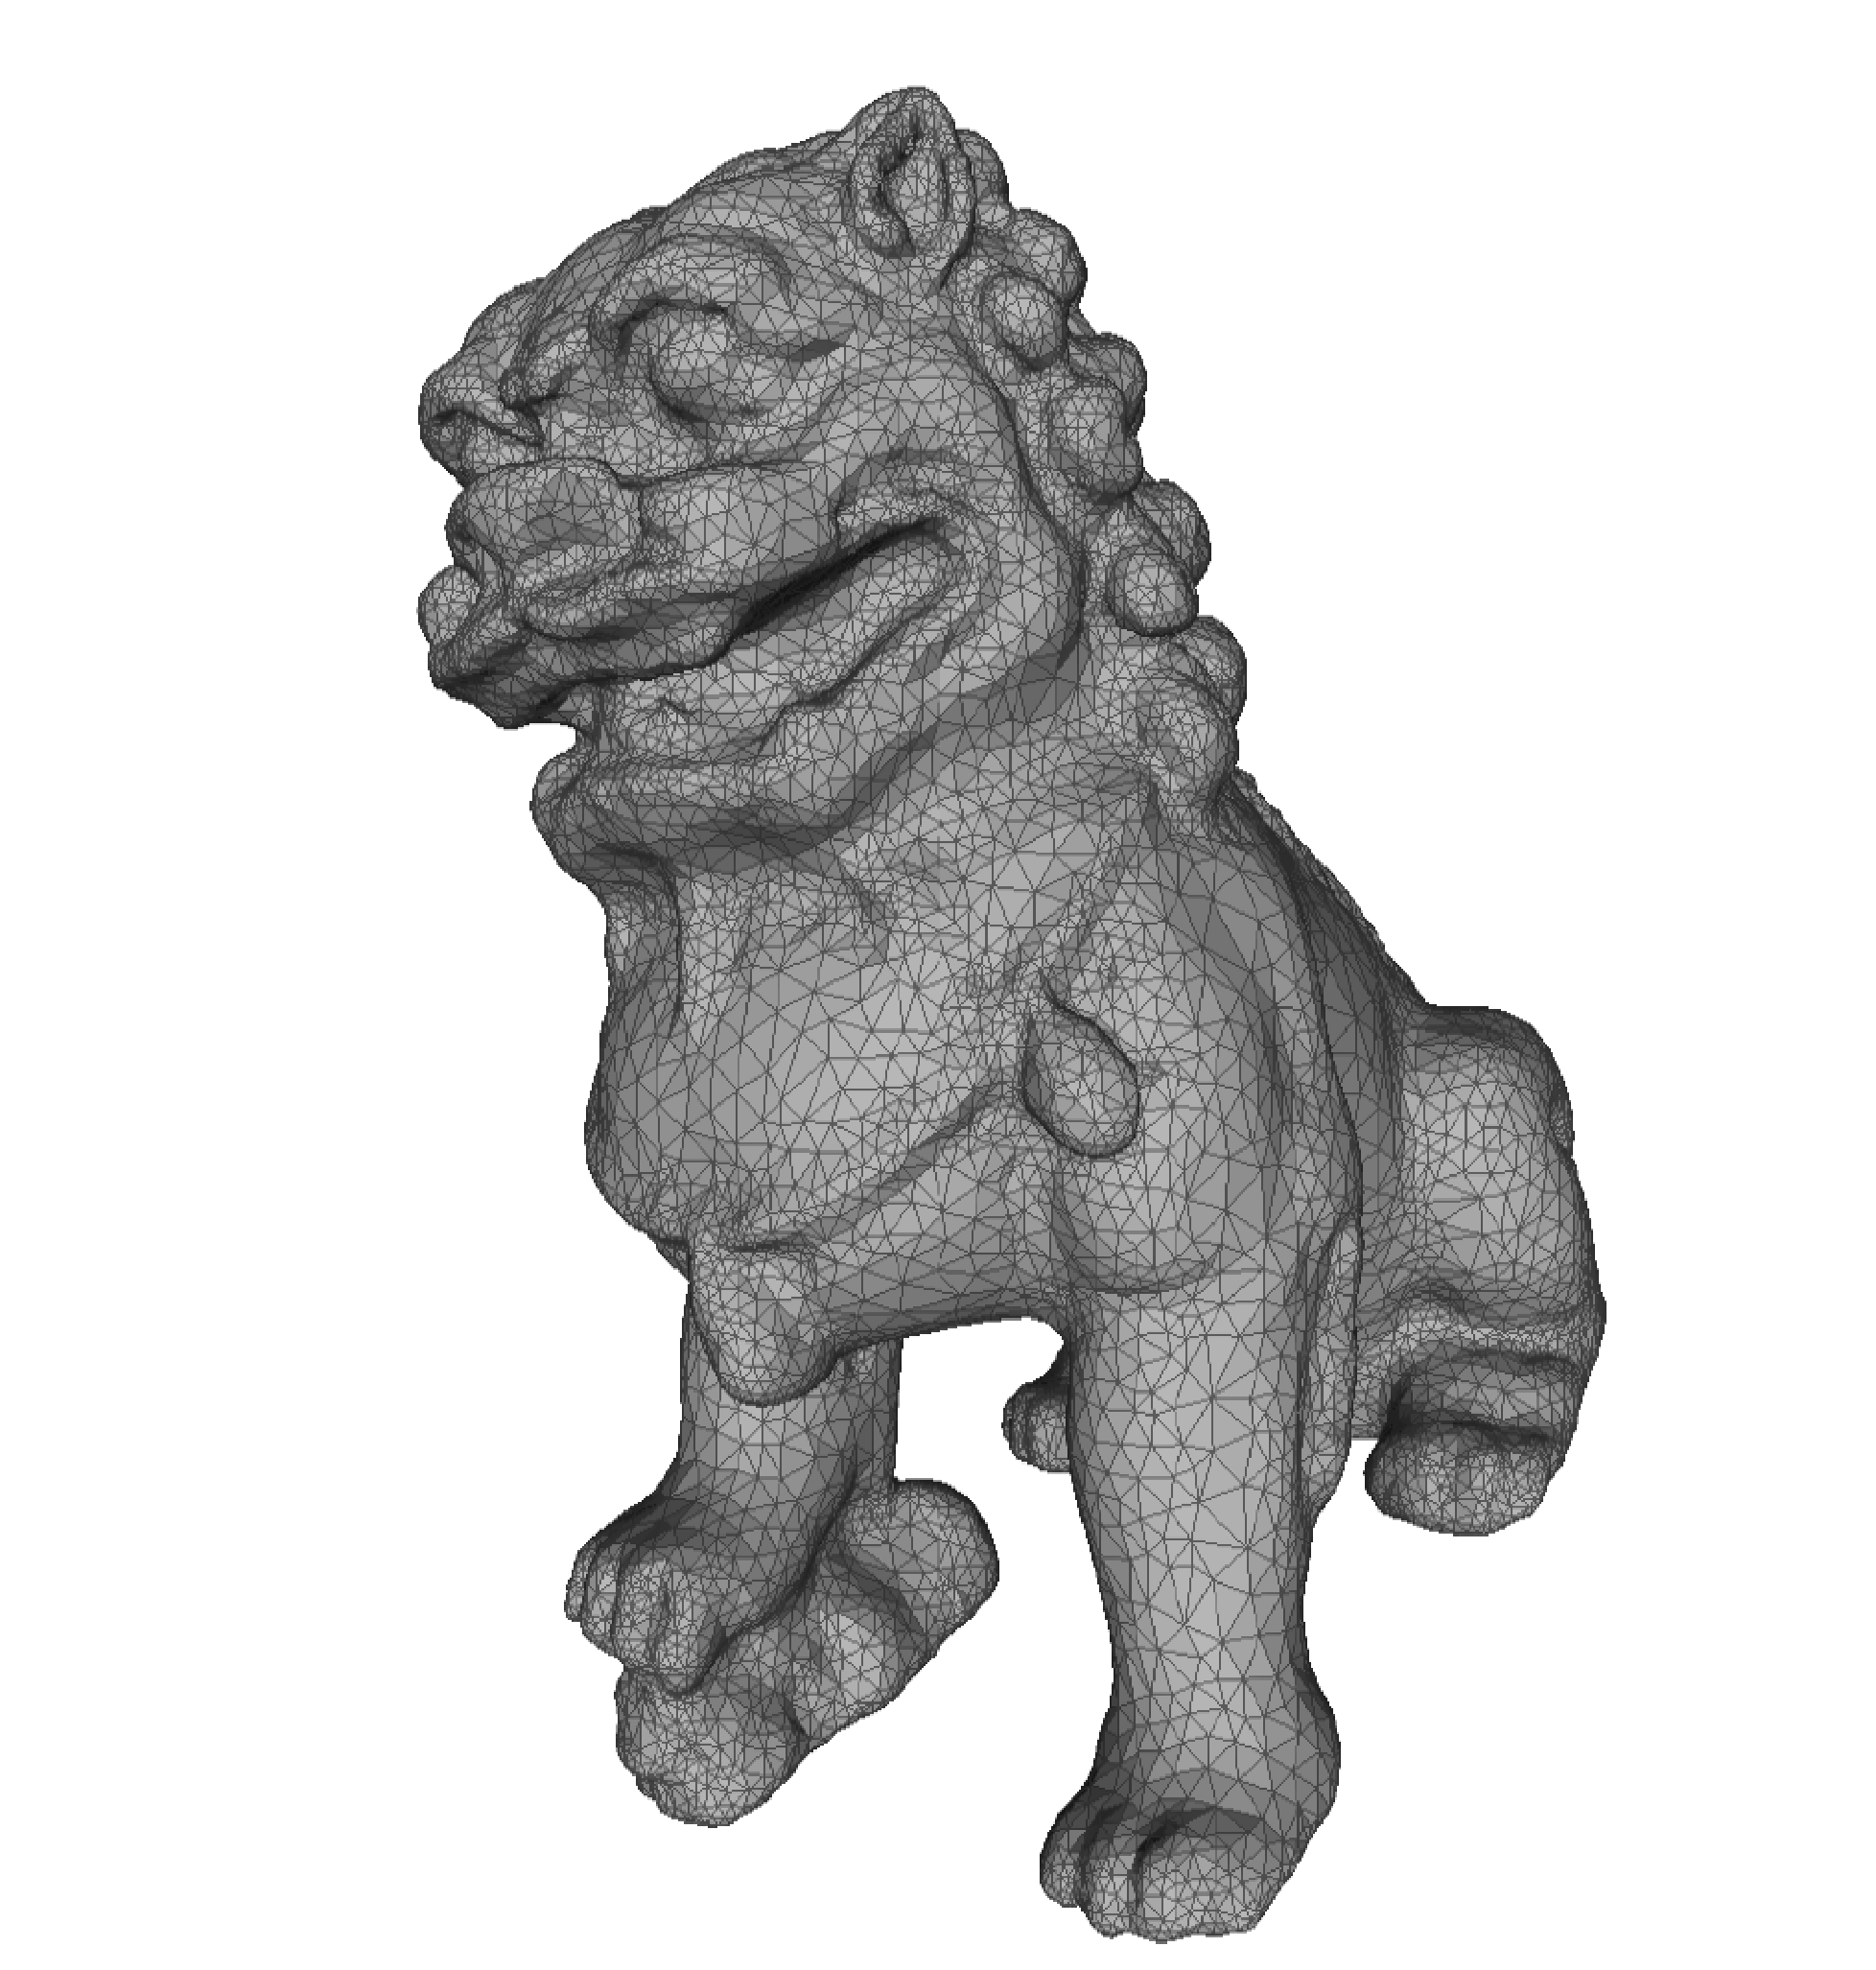
\includegraphics[width=0.7\textwidth]{Surface_reconstruction_3/APSS} % omit .eps suffix
    \end{ccTexOnly}
    \begin{ccHtmlOnly}
        <img width="70%" border=0 src="../Surface_reconstruction_3/APSS.jpg"><P>
    \end{ccHtmlOnly}
    % Title
    \begin{figure}[h]
        \caption{APSS reconstruction}
    \end{figure}
\end{center}

% The section below is automatically generated. Do not edit!
%START-AUTO(\ccDefinition)

\ccc{APSS_implicit_function} computes an implicit function that defines a Point Set Surface (PSS) based on moving least squares (MLS) fitting of algebraic spheres. See {\em Algebraic Point Set Surfaces} by Guennebaud and Gross \cite{Guennebaud07}.

The Surface Mesh Generation package makes copies of implicit functions, thus such a class must be lightweight and stateless.

%END-AUTO(\ccDefinition)

% The section below is automatically generated. Do not edit!
%START-AUTO(\ccInclude)

\ccInclude{CGAL/APSS_implicit_function.h}

%END-AUTO(\ccInclude)

\ccParameters

The full template declaration is:

% The section below is automatically generated. Do not edit!
%START-AUTO(\ccParameters)

template$<$  \\
class Gt$>$   \\
class \ccc{APSS_implicit_function};

\begin{description}
\item[Parameters:]
\begin{description}
\item[Gt]Geometric traits class. \end{description}
\end{description}

%END-AUTO(\ccParameters)

\ccIsModel

% The section below is automatically generated. Do not edit!
%START-AUTO(\ccIsModel)

Model of the ReconstructionImplicitFunction concept.

%END-AUTO(\ccIsModel)

\ccHeading{Design Pattern}

% The section below is automatically generated. Do not edit!
%START-AUTO(\ccHeading{Design Pattern})

A model of ReconstructionImplicitFunction is a Strategy \cite{cgal:ghjv-dpero-95}: it implements a strategy of surface mesh reconstruction.

%END-AUTO(\ccHeading{Design Pattern})

\ccTypes

% The section below is automatically generated. Do not edit!
%START-AUTO(\ccTypes)

\ccNestedType{Geom_traits}
{
Kernel's geometric traits.
}
\ccGlue
\ccNestedType{FT}
{
}
\ccGlue
\ccNestedType{Point}
{
}
\ccGlue
\ccNestedType{Iso_cuboid}
{
}
\ccGlue
\ccNestedType{Sphere}
{
}
\ccGlue
\ccNestedType{Point_with_normal}
{
}
\ccGlue
\ccNestedType{Normal}
{
}
\ccGlue
\ccNestedType{Vector}
{
}
\ccGlue

%END-AUTO(\ccTypes)

\ccCreation
\ccCreationVariable{fct}  %% variable name for \ccMethod below

% The section below is automatically generated. Do not edit!
%START-AUTO(\ccCreation)

\ccConstructor{APSS_implicit_function(InputIterator first, InputIterator beyond, unsigned int k, FT projection_error = 3.16e-4);}
{
Create an APSS implicit function from a point set.
Precondition: the value type of InputIterator must be convertible to \ccc{Point_with_normal}.
}
\ccGlue
\begin{description}
\item[Parameters:]
\begin{description}
\item[first]First point to add. \item[beyond]Past-the-end point to add. \item[k]Number of nearest neighbors. \item[\ccc{projection_error}]Dichotomy error when projecting point. \end{description}
\end{description}
\ccGlue
\ccConstructor{APSS_implicit_function(const APSS_implicit_function<Gt>& other);}
{
Copy constructor.
}
\ccGlue

%END-AUTO(\ccCreation)

\ccOperations

% The section below is automatically generated. Do not edit!
%START-AUTO(\ccOperations)

\ccMethod{APSS_implicit_function& operator=(const APSS_implicit_function<Gt>& other);}
{
operator =()
}
\ccGlue
\ccMethod{void setNofNeighbors(unsigned int k);}
{
}
\ccGlue
\ccMethod{Iso_cuboid bounding_box() const;}
{
Get the bounding box.
}
\ccGlue
\ccMethod{const Sphere& bounding_sphere() const;}
{
Get the surface's bounding sphere.
}
\ccGlue
\ccMethod{Sphere region_of_interest() const;}
{
Get the region of interest, ignoring the outliers. This method is used to define the OpenGL arcball sphere.
}
\ccGlue
\ccMethod{bool compute_implicit_function();}
{
You should call \ccc{compute_implicit_function}() once when points insertion is over. Return false on error.
}
\ccGlue
\ccMethod{FT operator()(const Point& p) const;}
{
[ImplicitFunction interface]
Evaluate implicit function for any 3D point.
}
\ccGlue
\ccMethod{Point get_inner_point() const;}
{
Get point inside the surface.
}
\ccGlue

%END-AUTO(\ccOperations)

\ccSeeAlso

\ccRefIdfierPage{Poisson_implicit_function}  \\

\ccExample

See \ccc{APSS_reconstruction.cpp} example.

\end{ccRefClass}

% +------------------------------------------------------------------------+
%%RefPage: end of main body, begin of footer
\ccRefPageEnd
% EOF
% +------------------------------------------------------------------------+

